\documentclass[11pt]{article}
\usepackage[utf8]{inputenc}
\usepackage[french]{babel}
\usepackage{graphicx}
\usepackage{caption}
\usepackage{fancyhdr} 
\usepackage{lastpage}
\usepackage{float}


\graphicspath{{./Images/}}

\renewcommand{\thesection}{\Roman{section}. }
\renewcommand{\thesubsection}{\Roman{section}.\arabic{subsection}}
\renewcommand{\thesubsubsection}{\Roman{section}.\arabic{subsection}.\alph{subsubsection} }

\setlength{\hoffset}{-18pt}        
\setlength{\oddsidemargin}{0pt}
\setlength{\evensidemargin}{0pt}
\setlength{\marginparwidth}{54pt}
\setlength{\textwidth}{494pt}
\setlength{\voffset}{-45pt}
\setlength{\marginparsep}{7pt}
\setlength{\topmargin}{0pt}
\setlength{\headheight}{13pt}
\setlength{\headsep}{15pt}
\setlength{\footskip}{35pt}
\setlength{\textheight}{680pt}

\pagestyle{fancy}

\renewcommand{\headrulewidth}{1pt}
\fancyhead[L]{\textsc{Tillings}}
\fancyhead[C]{}
\fancyhead[R]{\leftmark}

\renewcommand{\footrulewidth}{1pt}
\fancyfoot[L]{Rapport de projet}
\fancyfoot[C]{\textbf{\thepage/\pageref{LastPage}}}
\fancyfoot[R]{Equipe 132}


\title{Rapport Projet}
\author{\textsc{Marais} Lucas, \textsc{Boudeau} Benjamin}
\date{2020-2021}


\begin{document}





\begin{titlepage}
\centering

\includegraphics[scale=0.3]{ENSEIRB.png}
\\
\vspace*{1\baselineskip}
\LARGE{\textsc{Rapport de projet}}
\vspace*{0.8\baselineskip}
\rule{1\linewidth}{1pt}

\huge{\textbf{TILLINGS}}
\vspace*{1\baselineskip}
\rule{1\linewidth}{1pt}
\vspace*{1\baselineskip}
\LARGE{\textsc{Fillière Informatique - Semestre 5}}
\\

\large{18 Décembre 2020}
\vspace*{3\baselineskip}
\\
\centering
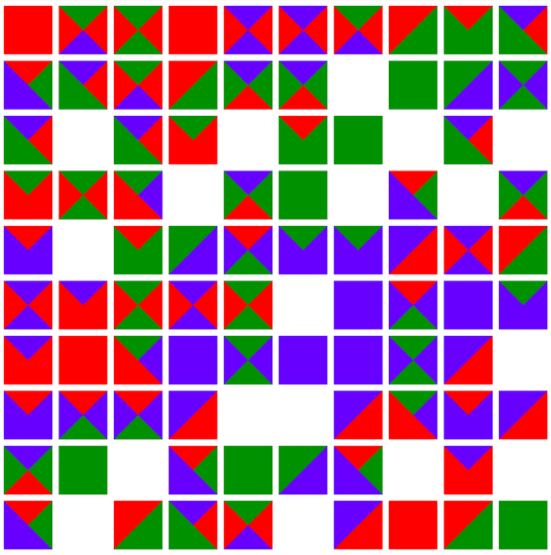
\includegraphics[scale=0.4]{tillings.png}
\\
\vspace*{4\baselineskip}

\begin{minipage}[b]{0.40\linewidth}
        \flushleft 
        \large
        Auteurs : 
        \\
        \textsc{Marais} Lucas
        \\
        \textsc{Boudeau} Benjamin
    \end{minipage} \hfill
    \begin{minipage}[b]{0.40\linewidth}
        \flushright 
        \large 
        Encadrants : 
        \\
        \textsc{Renault} David
        \\
        \textsc{Swartvagher} Philippe
    \end{minipage} \hfill

\end{titlepage}

\newpage

%\section*{Introduction}


%\newpage

\tableofcontents
\newpage

\section{Présentation du projet}
Dans le cadre de notre premier semestre de formation à l'ENSEIRB-MATMECA dans la filière informatique nous avons été amené à implémenter une simulation de partie d'un jeu de tuiles en langage C. 

\subsection{Principe du jeu}
Le jeu consiste à poser des tuiles sur un plateau de jeu,  une tuile est un carré découpé en 4 triangles ayant chacun une couleur. Chaque joueur se voit attribuer un nombre de tuiles qui composent son jeu et il doit les poser sur le plateau de jeu afin d'augmenter son score, le joueur ayant le plus haut score à la fin de la partie remporte le jeu. Pour placer une tuile le joueur doit faire attention à deux règles : \\ 
\begin{itemize}
    \item La règle de contiguïté selon laquelle chacun des triangles de la tuile posée doit correspondre au niveau des couleurs avec les autres tuiles dont elle est voisine.
    \item La règle de connexité selon laquelle une tuile ne peut être posée que si elle possède une arrête en commun avec au moins une tuile (exceptée la première tuile qui commence le jeu et qui est posée aléatoirement sur le plateau). \\
\end{itemize}

Voici un exemple de tuiles respectant ces deux règles :
\begin{figure}[H]
\centering
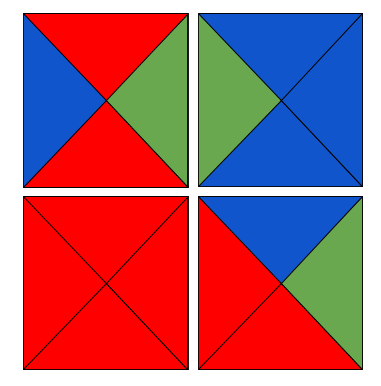
\includegraphics[scale=0.2]{Tuiles exemple.png}
\captionof{figure}{Exemple de tuiles}
\end{figure}

Chaque tuile posée rapporte 1 point au joueur et, si à la fin du jeu la tuile est la tuile centrale d'un motif, le joueur remporte un nombre de points correspondant au motif. La tuile centrale d'un motif est en fait une tuile monochrome où tous les triangles sont de la même couleur, voici deux exemples de motifs : 
\begin{figure}[H]
    \begin{minipage}[b]{0.40\linewidth}
        \centering 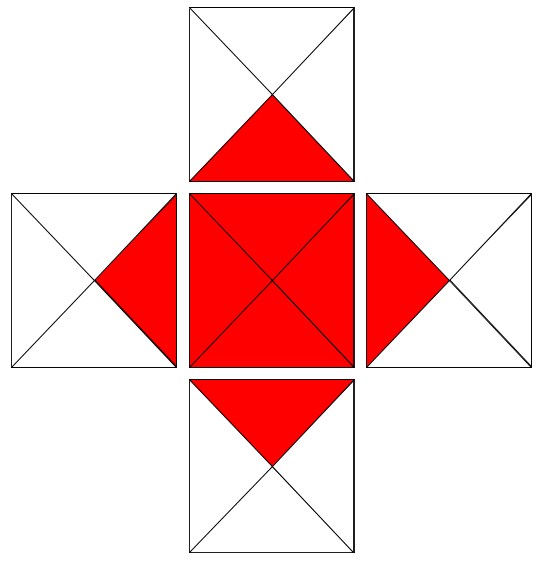
\includegraphics[scale=0.2]{Motif 34 points.png}
        \captionof{figure}{Motif rapportant 34 points}
    \end{minipage} \hfill
    \begin{minipage}[b]{0.40\linewidth}
        \centering 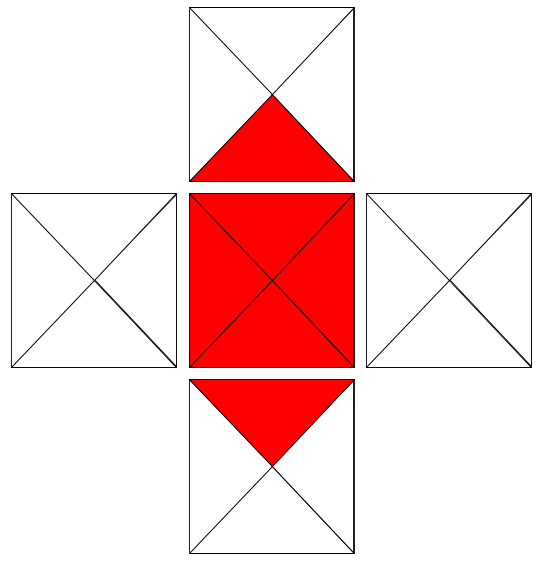
\includegraphics[scale=0.2]{Motif 20 points.png}
        \captionof{figure}{Motif rapportant 20 points}
    \end{minipage} \hfill
\end{figure}

Le but du projet est donc de créer un programme qui simule une partie de ce jeu en prenant plusieurs paramètres comme le nombre de joueurs ou la taille du plateau de jeu. 

\newpage

\subsection{Exemple de partie jouée}

Voici un exemple d'une partie jouée sur un plateau de taille 10 par 10 : 

\begin{figure}[H]
\centering
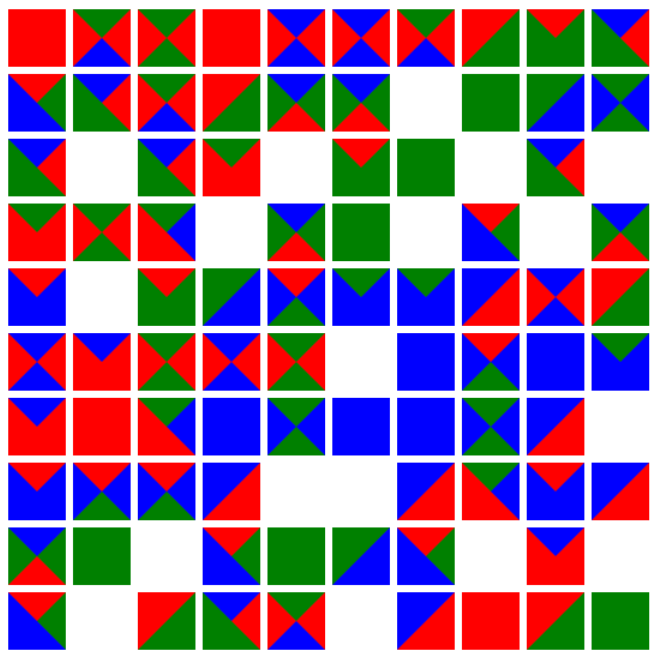
\includegraphics[scale=0.4]{Exemple -n 10.PNG}
\captionof{figure}{Exemple de partie}
\label{fig: exemplepartie}
\end{figure}

\section{Cadre de travail}
Pour optimiser notre travail, nous avons lors de chaque séance lancé une conférence Jitsi afin de partager nos écrans, nous discutions sur Discord en parallèle. Pendant presque l'intégralité du projet nous travaillions en pair-programming, c'est à dire qu'une seule personne codait une fonction ou un ensemble de fonctions et l'autre suivait et participait grâce au partage d'écran. Ainsi nous codions chacun notre tour et cela nous permettait de bien comprendre et d'interpréter de la même façon les structures et différents types manipulés lors du projet ainsi que la façon dont nous implémentions nos idées. En effet, avant l'écriture de chaque fonction, nous réfléchissions à la manière dont nous souhaitions traiter les contraintes et objectifs et nous élaborions un pseudo-code sur un fichier google-docs en commun. Il était donc important de bien comprendre le code C pour pouvoir l'utiliser de la bonne façon dans les autres fichiers.
\\

Lorsque les bases du projets on été codées, nous avons commencé à travailler en parallèle sur différents objectifs. Pour cela nous travaillions sur nos machines dans un répertoire personnel et nous faisions les \emph{commit} l'un après l'autre pour éviter au maximum les conflits de fusion sur le dépôt git.
\\

Au début de chaque séance et à la fin, nous faisions un point avec notre professeur référent pour être le plus efficace possible lors de la séance suivante. Également, nous tenions à jour un google-docs où nous notions les objectifs de chaque séance en début de séance, et les objectifs atteints ou non en fin de séance. Ainsi nous pouvions suivre facilement l'avancée du projet sans oublier certains détails.

\section{Implémentation du projet}

\subsection{Implémentation générale} \label{subsec: implementation}
L'implémentation générale de notre projet repose sur le déroulement d'une partie de jeu. Afin de lancer une partie, nous créons donc un deck selon la structure imposée dans le fichier \emph{tile.h} fourni avec le sujet, c'est à dire un tableau de \emph{deck\_pair} (Cf \ref{subsec: deck}). Ensuite nous transformons ce deck en une file de tuiles dont l'implémentation est fournie dans le fichier \emph{file.h}, que nous mélangeons et distribuons de façon équitable entre tous les joueurs (même nombre de tuiles). Pour cela nous créons un tableau de files de tuiles qui représentent la main de chaque joueur.
\\

Pour permettre aux joueurs de jouer, nous créons le plateau de jeu comme un tableau à double entrées dont chaque case est une \emph{board\_cell}, structure dont l'implémentation est fournie dans le fichier \emph{board.h}. Ainsi à une case du tableau, nous associons une tuile et un propriétaire, cela facilitera le calcul des scores en fin de partie. 
\\

Le premier joueur peut donc jouer et poser sa première tuile sur une case aléatoire du plateau. Ensuite la boucle de jeu commence : \newline
Le deuxième joueur joue avec sa tuile en tête de deck (celle qui est dans sa main). S'il peut la placer, il la positionne sur une case aléatoire parmi les positions disponible. Pour simplifier cette mise en oeuvre nous avons choisi que l'aléatoire choisirai toujours la première position trouvée. Au contraire, s'il ne peut pas la positionner, c'est à dire que le plateau dans l'état où il est ne permet pas le positionnement de la tuile dans le respect des règles de contiguïté et de connexité, le joueur \emph{skip} et sa tuile est déplacée en dernière position dans son deck. Ainsi les joueurs jouent les uns après les autres. \\ Le jeu s'arrête lorsqu'un joueur n'a plus de tuiles dans son deck ou si tous les joueurs ont skippé successivement.
\\

Il y a différentes manières de compter le score des joueurs. Une première façon, implémentée dans l'\emph{achiev0}, classe les joueurs selon le nombre de tuiles restantes dans leur deck à la fin de la partie, l'objectif étant d'en avoir le moins possible. Il est également possible de classer les joueurs selon le nombre de tuiles qu'ils ont posées en essayant de compléter des motifs définis dans le fichier \emph{pattern.h}, cette méthode de scoring est implémentée dans l'\emph{achiev1}.
\\

Afin d'organiser le code en plusieurs fichiers comprenant les fonctions spécifiques à un type (\emph{tile}, \emph{color}, \emph{file}, ...), nous utilisons des fichier ".c" et des fichiers ".h" permettant de faire référence dans un fichier au code présent dans un autre fichier. Le projet s'organise selon le graphe ci-dessous :

\begin{figure}[H]
\centering
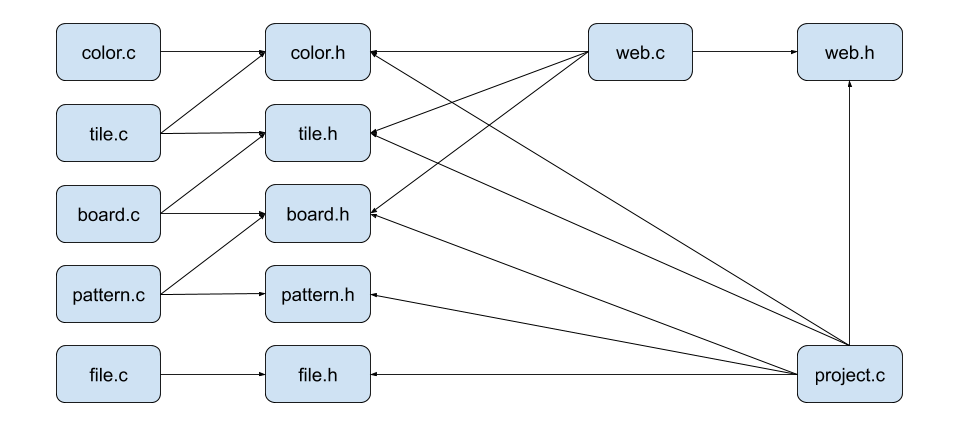
\includegraphics[scale=0.4]{graph include.png}
\captionof{figure}{Graphe des dépendances}
\end{figure}

\subsection{La gestion des couleurs} \label{subsec: color}
Dans le sujet du projet fourni par nos professeurs nous avions un fichier \emph{color.h} imposé, nous avons donc dû implémenter les couleurs en prenant en compte cette contrainte. Dans ce fichier on trouve une structure incomplète nommée \emph{color} ainsi que trois signatures de fonctions : 
\\

\begin{itemize}
\item Une fonction \emph{color\_name} qui prend un pointeur vers une \emph{color} et renvoie son nom.
\item Une fonction \emph{color\_cstring} qui prend un pointeur vers une \emph{color} et renvoie son code ANSI.
\item Une fonction \emph{color\_from\_name} qui prend un nom de couleur et renvoie un pointeur vers cette \emph{color}.
\\

\end{itemize}


Ainsi nous avons créé le fichier \emph{color.c} qui implémente cette structure et ces trois fonctions. La structure comporte deux champs de type chaîne de caractères, l'un se nomme \emph{name} et représente le nom associé à la couleur tandis que le second se nomme \emph{ANSI} et représente le code ANSI de la couleur. Ensuite, pour pouvoir utiliser ce code ANSI, dans une fonction \emph{printf} par exemple, nous avons modifié le contenu de ANSI en le remplaçant par une chaîne de caractères du type : "code ANSI de la couleur" + "première lettre de la couleur" + "code ANSI du blanc". Ainsi quand on affiche le code ANSI d'une couleur donnée, cela nous affiche la première lettre de la couleur dans la couleur associée. Le texte qui suit, s'il y en a, s'affiche en blanc et non de la couleur demandée précédemment, grâce au code ANSI du blanc donné après chaque code ANSI des couleurs.
\\

Notre première idée a été de créer les couleurs dans un fichier assez général de notre implémentation, par exemple au début du \emph{project.c}. Cependant nous avons ensuite compris le problème que nous allions rencontrer. Puisque \emph{color.h} fourni seulement une structure incomplète, nous ne pouvons donc pas créer de couleurs en dehors de \emph{color.c} qui connais lui les champs de la structure. C'est pourquoi nous avons créé un tableau de pointeurs \emph{color} dans le fichier \emph{color.c} qui contient des pointeurs vers les couleurs utilisées pendant le jeu, le but étant ensuite de ne manipuler que des pointeurs vers ces couleurs (comme dans les fonctions fournies par \emph{color.h}).

\begin{figure}[H]
\centering
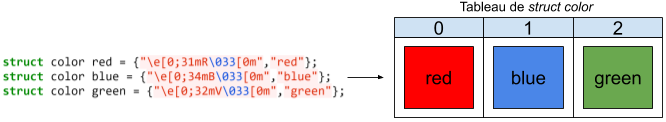
\includegraphics[scale=0.7]{Couleurs.png}
\captionof{figure}{Schématisation de la structure color}
\label{fig : color}
\end{figure}

Cette implémentation des couleurs à l'avantage de ne pas multiplier les \emph{color} dans la mémoire de la machine, chaque \emph{color} n'existe qu'une seule fois et on y fait référence dans le reste des fonctions. De plus, une couleur "vide", c'est à dire la couleur que pourrait prendre une tuile sans couleur est représentée par un pointeur \emph{NULL}. Cela rend la détection de tuiles vides plus facile puisque nous n'avons pas besoin de tester si le nom d'une des couleurs associées est "vide" par exemple, il nous suffit de comparer le pointeur \emph{color} avec le pointeur \emph{NULL}. \\  

Il nous est également impossible d'accéder aux champs d'une couleur autre part que dans \emph{color.c} puisque c'est le seul fichier qui connaît les champs de la structure \emph{color}, c'est pour cela que le sujet nous impose des fonctions qui prennent en entrée un pointeur vers une couleur pour ensuite nous donner son nom ou bien même son code ANSI. Grâce à ces deux fonctions nous pouvons effectuer un test d'égalité entre deux \emph{color} dans n'importe quel fichier qui inclut \emph{color.h}. La dernière fonction qui renvoie un pointeur vers une \emph{color} quand on lui donne le nom associé permet d'accéder aux pointeurs vers les \emph{color} dans n'importe quel fichier qui inclut \emph{color.h}. \\

Ainsi, nous possédons des fonction qui permettent d'accéder aux couleurs dans d'autres fichiers. L'implémentation des tuiles notamment utilise ces fonctions.

\subsection{La gestion des tuiles}
Le sujet nous fournit un fichier \emph{tile.h} comprenant une énumération de directions qui définissent les triangles des tuiles dans les directions respectives. Le sujet donne également une signature pour la structure \emph{struct tile}. Nous étions donc libre d'implémenter les tuiles comme nous le souhaitions. Nous avons choisi de représenter les tuiles par un tableau de taille 4 contenant des pointeurs (\emph{struct color*}) vers les couleurs définies précédemment, représentant ainsi les couleurs des 4 triangles constituant la tuile. De cette manière, l'énumération et la structure fonctionnent de pair pour connaître la couleur d'une tuile selon une direction, un élément de l'énumération correspond en effet à un indice du tableau comportant les couleurs de la tuile. \\

Les signatures fournies par le sujet demandent l'implémentation d'une fonction \emph{empty\_tile} qui retourne une tuile vide. L'utilisation des pointeurs est donc judicieuse, ainsi nous avons décidé qu'une tuile vide est un pointeur \emph{NULL} et cette fonction retourne donc un pointeur \emph{NULL}. \\

De la même manière, la fonction \emph{tile\_is\_empty}, dont la signature demande à ce qu'elle détermine si une tuile passée en paramètre est vide ou non, teste si la tuile en argument est un pointeur \emph{NULL} et retourne le résultat du test. \\

Le fichier \emph{tile.h} demande également l'implémentation d'une fonction comparant deux tuiles. Pour cela on compare les couleurs de chaque tuile dans chacune des directions. \\
Par exemple, sur la figure \ref{fig : tile_equals}, la fonction \emph{tile\_equals} renvoie 0 car les tuiles ne sont pas similaires. En effet, tous les tests fonctionnent jusqu'au test dans la direction \emph{WEST} où les couleurs ne sont pas similaires.

\begin{figure}[h]
\centering
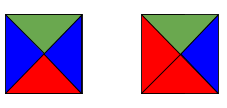
\includegraphics[scale=0.5]{tile_equals.png}
\captionof{figure}{Exemple d'utilisation de \emph{tile\_equals}}
\label{fig : tile_equals}
\end{figure}

Enfin, la structure \emph{tile} étant définie dans le fichier \emph{tile.c}, il est nécessaire d'avoir une fonction retournant la couleur d'une tuile dans une direction, ou plutôt un pointeur vers cette couleur. C'est l'objectif de la fonction \emph{tile\_edge}. Sur l'exemple de la figure \ref{fig : tile_equals}, \emph{tile\_edge} appelé sur la tuile de droite et dans la direction \emph{NORTH} renvoie un pointeur vers la couleur \emph{green} définie en figure \ref{fig : color}. \\

Une fois la structure des tuiles mise en place, nous pouvons maintenant travailler sur la structure des decks.

\subsection{La gestion des decks}\label{subsec: deck}
Le sujet nous impose les structures \emph{deck\_pair} et \emph{deck} :  \\

\begin{itemize}
\item Une \emph{deck\_pair} est composée d'un pointeur vers une tuile ainsi que d'un entier, il s'agit d'une tuile et de son nombre d'occurrences dans le jeu.
\item Un \emph{deck} est composé d'un tableau de \emph{deck\_pair} et d'un entier qui représente la longueur "utile" du tableau, c'est donc un ensemble de tuiles avec leur occurrence respective. \\
\end{itemize}
Dans les \emph{deck\_pair} et les \emph{deck} nous utilisons ainsi toujours des pointeurs vers des tuiles pour les même raisons que pour les couleurs : la structure dans \emph{tile.h} est incomplète. \\

\`A partir de ces structures nous devons arriver à avoir un \emph{deck} initial qui est l'ensemble de tuiles avec lesquelles les joueurs jouent. C'est le rôle de la fonction \emph{deck\_init} qui à partir d'un pointeur vers un \emph{deck} quelconque doit le transformer en un autre \emph{deck} qui est celui de base. Ainsi, quelque soit le \emph{deck} donné en entrée il deviendra forcement le deck générique que nous avons créé. \\

Pour effectuer cela, notre première idée était de créer un tableau de tuiles dans la fonction \emph{deck\_init} qui déterminerait les tuiles utilisées pendant le jeu, ensuite nous pourrions remplir le \emph{deck\_pair} avec ces tuiles en leur assignant un nombre d'occurrences pour ensuite remplir le \emph{deck} donné en entrée avec ces \emph{deck\_pair}. Cependant, les tuiles étant initialisées dans la fonction \emph{deck\_init} il est impossible de prendre des pointeurs vers ces tuiles car la valeur assignée aux cases mémoires correspondantes pourrait changer après l'appel d'autres fonctions dans la suite du programme. Pour palier à cela, un tableau de tuiles est créé en dehors de la fonction \emph{deck\_init}, le rôle de celle-ci est alors de construire des tuiles, de remplir le tableau de tuiles global avec ces tuiles pour ensuite créer des \emph{deck\_pair} avec des pointeurs vers les cases du tableau de tuiles global et enfin pouvoir initialiser correctement le \emph{deck} fourni en entrée. \\

Finalement, pour créer les tuiles nous avons besoin de pointeurs vers des couleurs, cela ne pose pas de souci puisque le fichier \emph{tile.c} inclut \emph{color.h} qui fourni la fonction \emph{color\_from\_name} qui permet d'obtenir des pointeurs vers les couleurs usuelles choisies (Cf \ref{subsec: color}). \\

Voici un schéma récapitulatif du fonctionnement de la fonction \emph{deck\_init} : 

\begin{figure}[h]
\centering
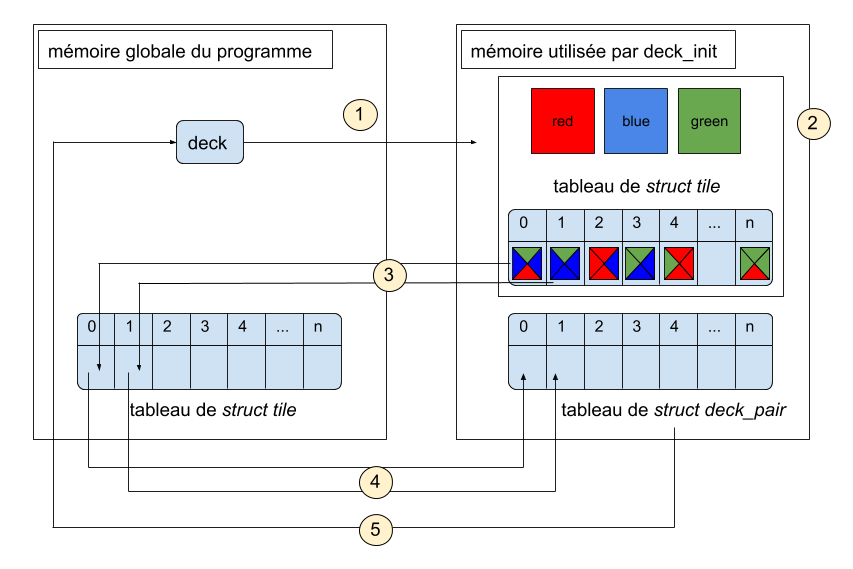
\includegraphics[scale=0.5]{deck_init.png}
\captionof{figure}{Schéma explicatif de \emph{deck\_init}}
\end{figure}

Explication du schéma : 
\begin{itemize}
\item L'étape 1 dans le schéma ci-dessus représente l'appel de la fonction, on lui donne un pointeur vers un \emph{deck} en argument. On remarque que le \emph{deck} fait partie de la mémoire globale ainsi que le tableau de tuiles vides dont nous avons parlé précédemment. 
\item L'étape 2 est la création d'un tableau de tuiles par la fonction, celui ci comprend les tuiles que nous avons choisi de donner aux joueurs pendant la partie (20 tuiles différentes).
\item L'étape 3 est celle où le tableau de tuiles de la mémoire globale est remplie avec les tuiles créées par la fonction \emph{deck\_init}.
\item  L'étape 4 est la répartition des tuiles (les pointeurs vers ces tuiles plus précisément) dans des \emph{deck\_pair} (l'entier qui constitue un \emph{deck\_pair} n'est pas représenté ici mais il est bel est bien initialisé en fonction d'une constante dans le programme).
\item L'étape 5 le tableau de \emph{deck\_pair} est mis dans le \emph{deck} donné en entré qui est maintenant correctement initialisé (comme pour les \emph{deck\_pair} l'entier associé à la structure \emph{deck} est donné par le biais d'une constante dans le programme). \\
\end{itemize}

\subsection{La création de files} \label{subsec: files}
\subsubsection{Utilisation de pointeurs void}
Pour gérer les decks des joueurs, le sujet nous suggérait l'utilisation du type file. Nous avons donc défini, dans un fichier \emph{file.h}, la structure liée aux files. Avant d'implémenter la structure et les fonctions liées au type file, nous avons réfléchi à l'utilisation que nous voulions en faire. Nous nous sommes dit que le type file serait utile pour géré les decks des joueurs comme indiqué par le sujet, mais également pour géré la file des joueurs. Nous avons donc implémenté le type file avec des pointeurs void c'est à dire des pointeurs qui ne pointent pas vers un type défini. \\ \\
Nous avons donc implémenté la structure \emph{file} avec : \\
\begin{itemize}
    \item \emph{queue} qui est un tableau de pointeurs void.
    \item \emph{size} qui est la taille "utile" du tableau \emph{queue}.
\end{itemize}

\subsubsection{Les fonctions du type file}
Dans tout le projet, nous avons considéré que la tête de la file était l'élément situé à l'indice 0 du tableau défini dans la structure, et que la queue de la file (le dernier élément) était l'élément situé à l'indice \(n\) du tableau avec \(n = size - 1\). \\
Ainsi nous avons codé les fonctions liées au type file : \\
\begin{itemize}
    \item la fonction \emph{push} qui ajoute un élément à la queue de la file.
    \item la fonction \emph{top} qui retourne l'élément en tête de file.
    \item la fonction \emph{pop} qui supprime l'élément en tête de file et le retourne. \\
\end{itemize}

\begin{figure}[H]
\centering
\fbox{
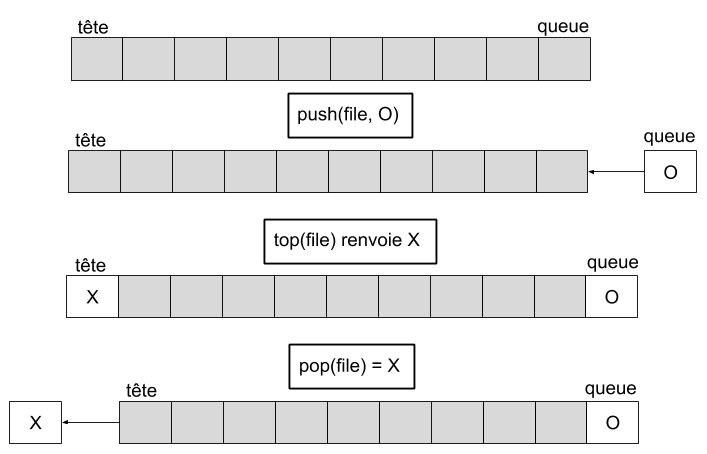
\includegraphics[scale=0.4]{Structure file.png}
}
\captionof{figure}{Fonctions principales du type file}
\end{figure}

Dans la boucle de jeu, nous avons besoin de mélanger les tuiles avant de les distribuer, ainsi nous avons ajouté deux autres fonctions : \\
\begin{itemize}
    \item la fonction \emph{mix} qui mélange une file. Pour cela nous donnons en argument de la fonction l'adresse de la file à mélanger. La fonction choisi un élément aléatoire de la file et le place à l'indice 0, puis elle prend un élément aléatoire entre les indices 1 et \(size - 1\) et elle le place en deuxième position, et ainsi de suite. Ainsi elle mélange aléatoirement la file.
    \item la fonction \emph{distribute} distribue la file entre tous les joueurs. Le sujet imposait des decks de taille maximale 200, c'est à dire qu'un joueur ne peut pas avoir plus de 200 tuiles dans son deck. Ainsi la fonction distribue une carte dans chacune des mains des joueurs (les mains des joueurs sont détaillés dans la sous-sous-section \ref{subsec: player}), puis une deuxième et ainsi de suite jusqu'à ce qu'il n'y ait plus de carte à distribuer (ou plus assez pour en redonner une à chaque joueur) ou que les joueurs aient déjà 200 tuiles. \\
\end{itemize}

\subsection{La gestion du plateau de jeu}
Lors de l'achievement 0 le plateau était un tableau à double entrées de tuiles cependant l'achievement 1 demande aux tuiles posées d'avoir un propriétaire ainsi nous avons changé notre manière d'implémenter le plateau de jeu. La structure \emph{board\_cell} comporte deux champs : un pointeur vers une tuile et un entier. En effet, les joueurs sont en fait des entiers (Cf \ref{subsec: player}), ainsi l'entier d'une \emph{board\_cell} est l'entier qui représente le joueur qui l'a posée. Le plateau est alors représenté par un tableau de \emph{board\_cell}. En ce qui concerne sa taille, celle-ci ne pouvant pas être initialisée à partir d'une variable dans le langage C nous avons choisi de l'initialiser avec une taille maximale c'est à dire 50 par 50 dans notre cas. Cela ne pose aucun souci pour le déroulement du jeu, la taille du plateau choisie par le joueur déterminera la zone du plateau à tester pour le positionnement des tuiles et les emplacements super-flux resteront avec leur valeur de départ à savoir une tuile vide (un \emph{NULL}). Voici un schéma qui explique comment est géré le problème de taille maximale du plateau de jeu (avec une taille maximale de 10 par 10 ici pour garder la lisibilité) :

\begin{figure}[H] 
\centering
\fbox{
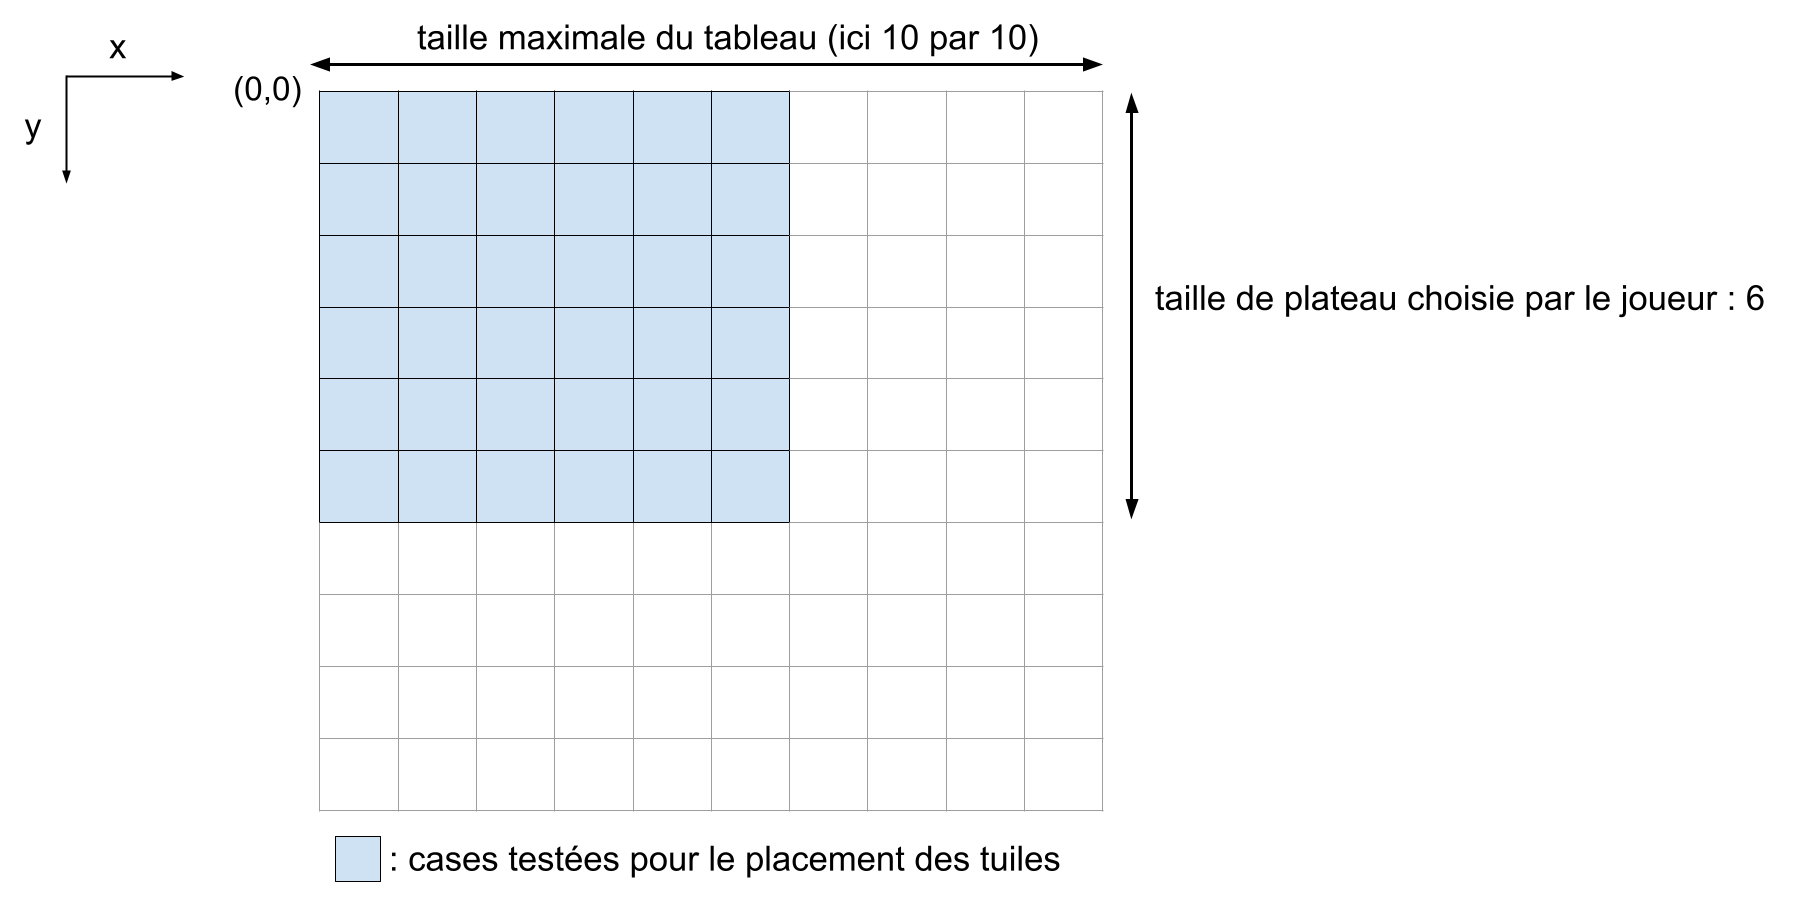
\includegraphics[scale=0.28]{taille plateau.png}
}
\captionof{figure}{Solution vis a vis de la taille variable d'un tableau}
\label{fig: boardsize}
\end{figure}


En ce qui concerne les coordonnées nous avons choisi de mettre l'origine en haut à gauche du tableau, l'origine correspond à l'élément du tableau en indice (0,0). De plus l'axe des abscisses (x) est dirigé vers la droite et l'axe des ordonnées (y) vers le bas. Tout ceci est représenté sur la figure \ref{fig: boardsize}. \\

La structure \emph{board\_cell} dont nous avons parlé précédemment a été placée dans un fichier \emph{board.h} qui contient la structure et les prototypes des fonctions utiles au plateau :

\begin{itemize}
\item La fonction \emph{owner} qui renvoie l'entier correspondant au propriétaire de la tuile (\emph{board\_cell}) donnée en entrée.
\item La fonction \emph{tile} qui renvoie le pointeur vers la tuile associé à la \emph{board\_cell} fournie en entrée.
\item La fonction \emph{change\_owner} qui prend un entier et une \emph{board\_cell} et remplace la valeur du champ correspondant au propriétaire de la \emph{board\_cell} par l'entier donné en entrée.
\item La fonction \emph{change\_tile} qui prend un pointeur vers une tuile ainsi qu'une \emph{board\_cell} et qui remplace le champ correspondant à la tuile dans la \emph{board\_cell} par la tuile fournie en entrée. \\
\end{itemize}

La structure \emph{board\_cell} est donnée dans \emph{board.h}. Il aurait donc été possible de se passer de ces 4 fonctions et d'agir sur la structure directement avec des affectations sur \emph{board\_cell.owner} par exemple. Cependant, nous avons choisi de créer ces fonctions pour garder de la clarté dans le code, une fonction étant plus parlante qu'une affectation. \\

Le fichier \emph{board.h} contient d'autres prototypes dont l'implémentation se trouve dans \emph{board.c}. Parmi ces fonctions on retrouve les deux fonctions liées aux tests sur le placement d'une tuile que nous verrons dans la sous-section \ref{subsec: tests}. La dernière fonction est \emph{draw\_board} qui prend un tableau à deux dimensions de \emph{board\_cell} en entrée et affiche le contenu dans le terminal, pour chaque case elle affiche "couleur nord, couleur sud, couleur est, couleur ouest, propriétaire", cette fonction a été utilisée pour vérifier que les règles de contiguïté et de connexité étaient bien respectées. \\

Nous disposons d'une seconde méthode de représentation graphique du plateau de jeu. Il s'agit de la fonction \emph{web\_export} qui créé un fichier HTML dans le dossier de l'exécutable afin d'afficher une représentation du plateau en fin de partie. La figure \ref{fig: exemplepartie} en est un exemple d'utilisation. Par la suite nous avons rajouté l'affichage de l'entier correspondant au propriétaire à l'intérieur des cases du tableau.

\subsection{La boucle de jeu}
\subsubsection{Déroulement d'une partie}
Comme expliqué dans la section \ref{subsec: implementation}, une partie débute par la distribution des decks aux joueurs. Ensuite le premier joueur pose sa tuile à une position aléatoire du plateau. La boucle de jeu commence alors. En effet, tant que tous les joueurs n'ont pas skippé successivement, c'est à dire tant que le compteur des joueurs ayant skippé n'est pas égal au nombre de joueur dans la partie en cours, chaque joueur joue l'un après l'autre en respectant les règles de contiguïté et de connexité. La tuile en tête de file du joueur actif est donc passée en paramètre des fonctions de tests afin d'analyser s'il est possible de la placer sur le plateau de jeu (Cf \ref{subsec: tests}). Si c'est le cas, alors le compteur des joueurs ayant skippé est remis à 0 et la tuile est placée. Ensuite, soit le joueur possède d'autres tuiles et on passe au joueur suivant, soit il vient de positionner sa dernière tuile et la partie est terminée, on peut alors comptabiliser les scores. Si la tuile n'a pas pu être placée, alors elle est remise en fin de file du joueur actif et on passe au joueurs suivant, le compteur des joueurs ayant skippé augmente alors de 1. \\
La figure \ref{fig : boucle} illustre le déroulement d'une partie avec la boucle de jeu :

\begin{figure}[H] 
\centering
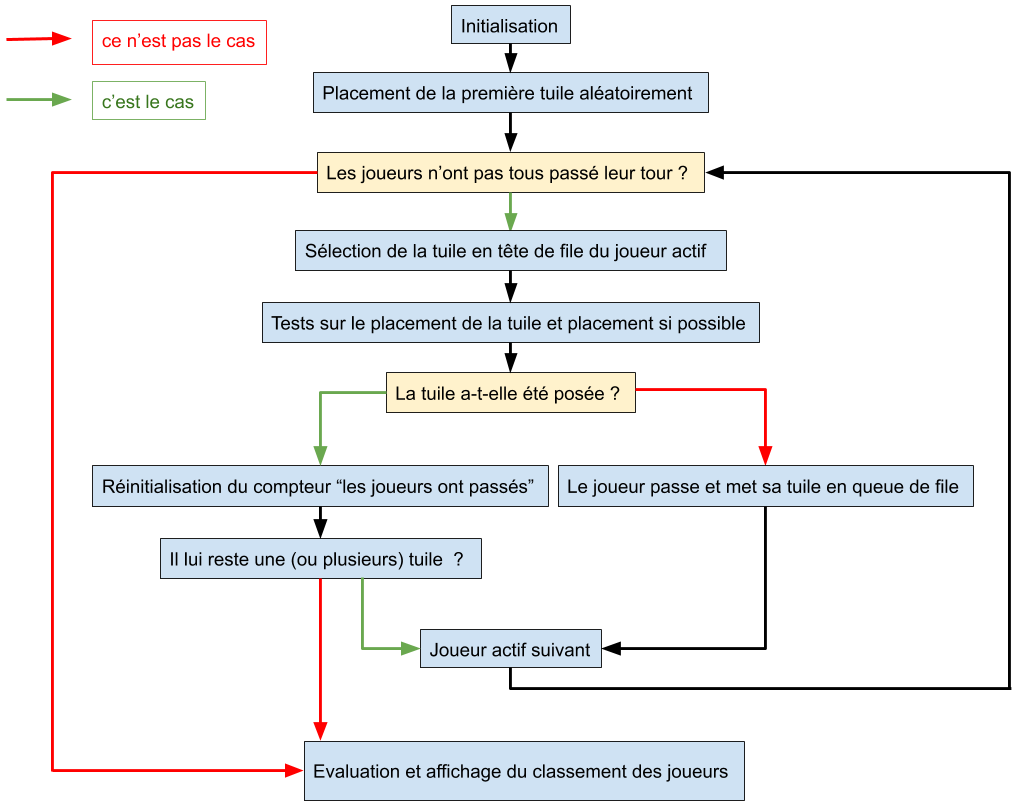
\includegraphics[scale=0.45]{Boucle jeu.png}
\captionof{figure}{Boucle de jeu}
\label{fig : boucle}
\end{figure}

\subsubsection{Les tests sur le plateau} \label{subsec: tests}
Cette section détaille les choix d'implémentation de la fonction \emph{test\_position} (code en annexe) qui prend en argument un plateau de jeu, une tuile et les coordonnées d'une case sur le plateau et qui renvoie si la tuile peut être placée à cet endroit. Cela reviens à tester si la case est vide dans un premier temps afin de savoir s'il est possible d'y placer une tuile et d'éviter de faire des tests inutiles. Si la tuile est vide il faut alors tester les règles de contiguïté et de connexité. 
\\

Les tests de connexité et de contiguïté ne sont pas compliqués mais il faut faire attention aux cas limites. L'idée la plus facile à mettre en place est une batterie de tests de cas de limites et faires les tests en conséquence mais cela n'est pas très optimal au niveau de la longueur du programme. C'est pourquoi nous avons créé le tableau de booléens \emph{direction}. Celui-ci possède 4 cases, une pour chaque direction. Ainsi, si le booléen dans une direction donnée (appelée \emph{dir} ici) du tableau est TRUE (1 en langage C), alors il faut tester si la couleur de la tuile en argument dans la direction \emph{dir} est la même que celle de la tuile présente sur le plateau dans la direction \emph{dir} par rapport à l'emplacement testé.
\\
\begin{figure}[H] 
\centering
\fbox{
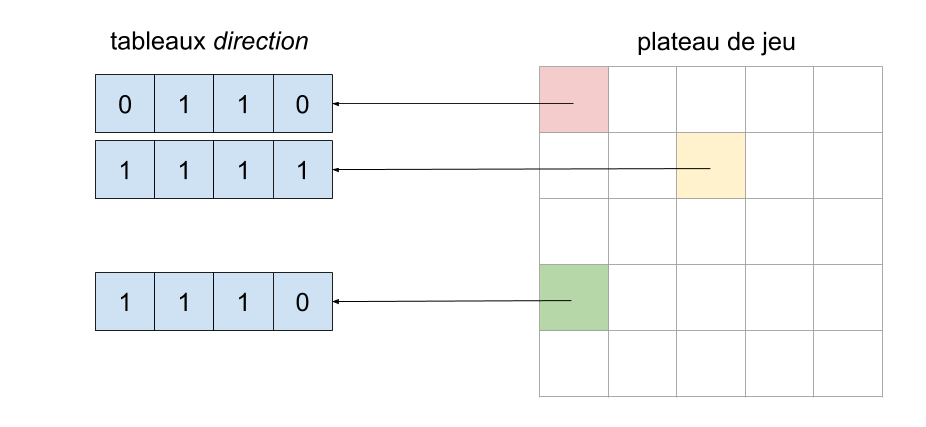
\includegraphics[scale=0.4]{direction.png}
}
\captionof{figure}{Exemples de tableaux \emph{direction}}
\label{fig: position}
\end{figure}

Par exemple, si nous testons le positionnement d'une tuile sur la position (x,y) = (0,0) (tuile rouge sur la figure \ref{fig: position}), alors le tableau de booléens des directions à tester devient : {0, 1, 1, 0} car les directions à tester sont \emph{SOUTH} et \emph{EAST}. Ainsi il faut comparer la couleur de la tuile à placer dans la direction \emph{SOUTH} et la couleur de la tuile en position (x,y+1) = (0,1) du plateau dans la direction \emph{NORTH}. Il faut également comparer la couleur de la tuile à placer dans la direction \emph{EAST} et la couleur de la tuile en position (x+1,y) = (1,0) du plateau dans la direction \emph{WEST}. De même, si la tuile à tester est en plein milieu du plateau de jeu comme la tuile jaune de la figure \ref{fig: position} par exemple, alors il faut tester toutes les directions et ainsi de suite pour tous les cas limites. \\

Le tableau de booléens permet donc d'intégrer les cas limites à la boucle générale des tests. De cette manière, au début de \emph{test\_position} nous faisons les tests des cas limites qui décident dans quelles directions nous avons besoin d'effectuer les tests de contiguïté pour que la tuile puisse être placée. Ensuite, on a une boucle \emph{for} qui pour chaque direction, si cette direction doit être testée (TRUE dans le tableau de booléens), alors on regarde si les règles de contiguïté et de connexité sont respectées entre la tuile donnée et la tuile dans la direction donnée par l'incrémenteur de la boucle \emph{for}. Cependant, si la tuile est comparée avec celle du dessus on va devoir regarder le \emph{NORTH} de la tuile en argument et le \emph{SOUTH} de la tuile du dessus. Il faudrait donc, pour chaque cas différent, faire les tests sur les couleurs de la tuile à placer (dans une direction) et de la tuile déjà présente sur le plateau (dans la direction opposée). Afin de gérer toutes les situations dans une même boucle et éviter de faire les tests au cas par cas, nous avons implémenté les fonctions \emph{opposite\_direction}, \emph{direction\_x} et \emph{direction\_y} : \\
\begin{itemize}
    \item La fonction \emph{opposite\_direction} prend en argument une direction et renvoie la direction opposée.
   \item Les fonctions \emph{direction\_x} et \emph{direction\_y} donnent les variations de coordonnées respectivement en abscisses et en ordonnées qu'il faut effectuer pour accéder à la tuile située sur le plateau dans la direction donnée en argument. \\
\end{itemize}

Lorsqu'avec ces fonctions nous avons les coordonnées de la tuile présente sur le plateau à comparer avec la tuile donnée en argument, il faut d'abord vérifier qu'elle ne soit pas vide sinon aucun test n'est à faire. Si la tuile existe, il suffit de comparer les couleurs de la tuile à placer et la tuile à coté (on utilise \emph{opposite\_direction} pour connaître les directions à comparer). Pour tester la règle de connexité, nous avons ajouté un compteur qui compte le nombre de tuiles non vides à côté de l'emplacement testé. Par exemple, si le compteur vaut 0 après la boucle des tests, alors on ne peut pas placer la tuile ici, car la règle de connexité ne serait pas respectée. \\

Cette fonction de tests est utilisée par \emph{tile\_placement} pour tester toutes les cases du plateau, cette fonction prend en argument une tuile et un plateau de jeu et teste pour chaque position du plateau de jeu (en parcourant toutes les lignes une par une) si la tuile donnée peut être placée ici. Si c'est le cas, la fonction la place et renvoie 1 sinon elle ne la place pas et renvoie 0.

\subsubsection{Les joueurs}\label{subsec: player}
Comme dit en \ref{subsec: files} au début de notre réflexion sur l'implémentation du jeu nous voulions gérer les joueurs et leur score à l'aide d'une file d'entiers, la main d'un joueur à l'aide d'une file de tuiles et l'ensemble des mains via une file de files de tuiles. Cependant, cette implémentation s'est révélée compliquée à mettre en place pour quelque chose de pas vraiment optimal en terme d'espace utilisé et de nombre d'opérations. Nous avons trouvé une façon beaucoup plus simple et moins coûteuse pour gérer les joueurs : chaque joueur est un entier. En effet, cela permet de remplacer la file d'entier du score par un tableau d'entier et on accède au score d'un joueur en accédant à la case d'indice "entier associé au joueur en question" du tableau des scores. De plus, les mains des joueurs sont alors des files de tuiles et l'ensemble des mains constitue un tableau. C'est ce tableau que nous donnons en argument à la fonction \emph{distribute}. Les tableaux ne pouvant pas être initialisés selon une taille variable, nous avons donc initialisé ce tableau avec une taille correspondant au nombre maximal de joueurs possible. Le jeu se comporte correctement grâce à l'incrémentation du joueur actif modulo le nombre de joueur choisi et également grâce à la fonction \emph{distribute} qui ne distribue qu'à un nombre limité de joueurs (le nombre choisi par l'utilisateur). La figure \ref{fig : struct joueurs} schématise la solution des tableaux pour gérer les structures associées aux joueurs. 
\\

\begin{figure}[H] 
\centering
\fbox{
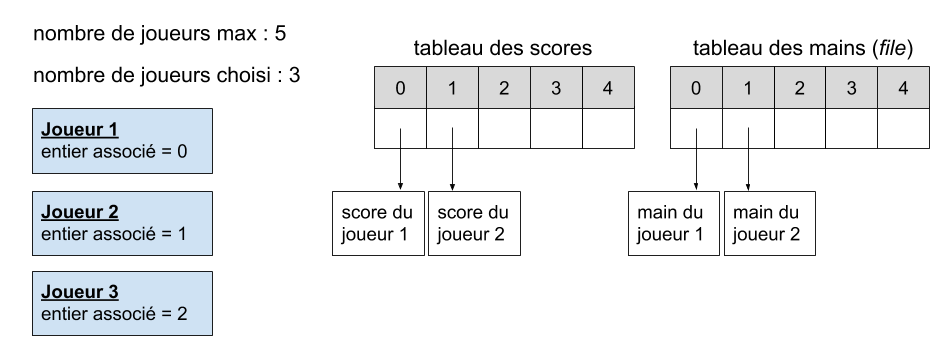
\includegraphics[scale=0.5]{Joueurs.png}
}
\captionof{figure}{Structures liées aux joueurs}
\label{fig : struct joueurs}
\end{figure}

Pour gérer le joueur actif nous n'avons pas besoin d'une file d'entiers et d'effectuer une rotation de ces éléments, il nous suffit à chaque tour de boucle de jeu d'incrémenter l'entier représentant le joueur actif modulo le nombre de joueur choisi par l'utilisateur pour éviter les dépassements. Ainsi nous avons une rotation des joueurs actifs, la figure \ref{fig : joueur actif} illustre cette rotation avec une partie à 3 joueurs.
\\
\begin{figure}[H] 
\centering
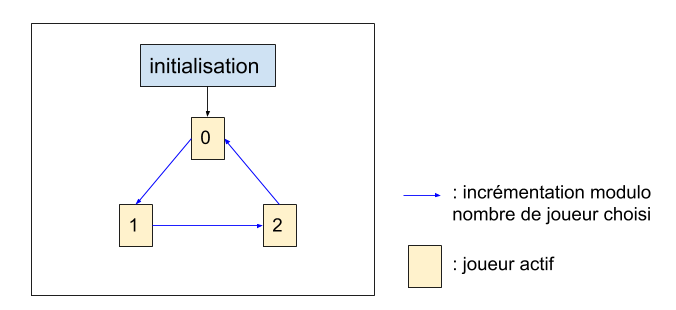
\includegraphics[scale=0.5]{Joueurs actifs .png}
\captionof{figure}{Rotation du joueur actif dans une partie à 3 joueurs}
\label{fig : joueur actif}
\end{figure}



\subsubsection{Le score} \label{subsec: score}
Dans l'achievement 0  la seule manière de gagner des points est de poser des tuiles. Ainsi comme au début du jeu chaque joueur a le même nombre de tuiles dans sa main il suffit juste de compter le nombre de tuiles restantes dans la main des joueurs en fin de partie et de ranger les joueurs dans le sens croissant du nombre de tuiles restantes pour obtenir le classement de la partie. Cependant, l'achievement 1 rajoute, comme il sera expliqué en détail dans la partie \ref{subsec: patterns}, un système de motifs qui peuvent rapporter des points aux joueurs. Nous avons donc dû revoir notre système de comptage de point : le score est géré par un tableau d'entiers, chaque case représente le score d'un joueur et pour y accéder on utilise comme pour les mains des joueurs l'entier associé au joueur comme un indice pour accéder à le bonne case du tableau. Le score du joueur actif est alors incrémenté d'une certaine valeur, gérée par une constante (celle-ci vaut 1 dans notre programme), à chaque fois qu'il pose une tuile. Ensuite, en fin de partie le programme évalue les points rapportés par les motifs afin de ranger les joueurs dans l'ordre décroissant du score et obtenir le classement de la partie. 


\subsection{L'ajout de motifs} \label{subsec: patterns}
\subsubsection{Les motifs}
Pour complexifier le code mais surtout pour rendre une partie de jeu plus intéressante, le sujet, par l'intermédiaire de l'achievement 1, nous proposait d'implémenter des motifs qui rapportent un certain nombre de points aux joueurs. Ainsi un joueur qui place une tuile centrale (tuile colorée par une seule et unique couleur) et que le déroulement de la partie entraîne l'apparition d'un motif autour de cette tuile, remporte les points associés au motif formé. Nous avons implémenté trois motifs différents valant respectivement 34, 20 et 10 points pour le propriétaire de la tuile centrale. Et deux des trois motifs peuvent varier selon l'orientation ce qui fait au total 7 motifs différents.

\begin{figure}[H] 
\centering
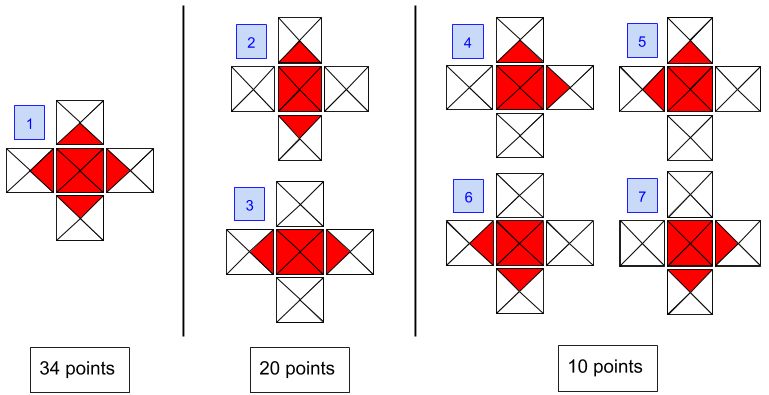
\includegraphics[scale=0.5]{Ensemble des motifs.png}
\captionof{figure}{Ensemble des motifs}
\label{fig : motifs}
\end{figure}

\subsubsection{Détection des motifs sur le plateau de jeu}
Pour trouver les motifs sur le plateau de jeu en fin de partie, nous avons implémenté une structure \emph{pattern\_score} qui prend un pointeur vers une fonction qui correspond à la fonction retrouvant un motif donné et un entier qui correspond au score de ce motif. Ensuite nous avons codé dans le fichier \emph{pattern.c} l'ensemble des 7 fonctions des motifs, par exemple la fonction \emph{pattern1} appelée sur la tuile à la position (x,y) du plateau de jeu, regarde si la tuile en (x,y) est monochrome et analyse si les 4 côtés des 4 tuiles dans les directions\emph{NORTH, SOUTH, EAST, WEST} sont de la même couleur que la tuile centrale. Cette fonction cherche donc à détecter le motif rapportant 34 points.\\

Pour cela nous avons créé des fonctions auxiliaires : \emph{is\_monochrome} et \emph{same\_color}.
\emph{is\_monochrome} retourne la couleur de la tuile passée en paramètre si cette-dernière est composée d'une unique couleur.
\emph{same\_color} analyse si la tuile à la position (x,y) du plateau (x, y et le plateau sont passés en paramètres) est monochrome et elle renvoie 1 si les côtés des tuiles dans deux directions d1 et d2 données en arguments sont de la même couleur que la tuile en (x,y). Elle renvoie 0 sinon. \\

Ainsi, \( \forall i \in {\{1,2,3,4,5,6,7\}} \), les fonctions \emph{pattern'i'} appellent la fonction \emph{same\_color} dans les directions souhaitées pour la détection du motif i. Par exemple \emph{pattern7} renvoie 1 si \emph{same\_color} vaut 1 dans les directions \emph{SOUTH, EAST}, car elle teste le motif 7 de la figure \ref{fig : motifs}.

\subsubsection{Organisation du code}
Enfin, pour organiser le code et pouvoir ajouter des motifs facilement, nous avons créé un tableau de \emph{struct pattern\_score} et nous parcourons ce tableau en faisant les tests par ordre de priorité (le motif 1 est testé en premier, puis le 2, etc...) dans une fonction générale nommée \emph{pattern}. Ainsi pour ajouter un motif il suffit d'écrire la fonction de recherche de ce motif et de l'ajouter dans le tableau avec les points associés au nouveau motif. Cette fonction renvoie le score associé au motif qu'elle a trouvé pour la position testée et donnée en paramètre, elle renvoie 0 si elle n'a trouvé aucun motif. Ainsi, comme expliqué en \ref{subsec: score}, nous pouvons facilement calculé le score d'un joueur en fin de partie.

\subsection{Complexité et Correction}
\subsubsection{L'utilisation des pointeurs}
L’approche de structures incomplètes et la manipulation de pointeurs est une façon d'optimiser nos fonctions et donc l'ensemble du programme. En effet, pour les couleurs et les tuiles par exemple, il est cohérent de ne manipuler que des pointeurs plutôt que de créer une instance d’un \emph{struct color} pour chaque couleur. Ainsi, il nous suffit de faire référence à la couleur créée dans color.c avec les pointeurs et non d'utiliser des cases mémoire en plus. La méthode est exactement la même pour les tuiles. Par exemple, les joueurs ayant une tuile en commun ne manipulent en fait qu'une seule et unique tuile par l'intermédiaire de son adresse mémoire. Les joueurs manipulent donc des adresses plutôt que des tuiles. La complexité en espace est donc nettement améliorée.

\subsubsection{Les fonctions \emph{test\_position} et \emph{tile\_placement}}
Dans l'ensemble de notre projet, les fonctions les plus complexes sont celles qui établissent des tests sur le plateau de jeu. En effet, les fonctions qui ne dépendent pas de la taille du plateau de jeu, sont soit de complexité \( \theta(1) \), soit de complexité \( \theta(board\_size^2) \) car elles s'arrêtent lorsqu'elles ont parcouru l'ensemble du plateau de jeu. Nous détaillerons donc les complexités des fonctions \emph{test\_position} et \emph{tile\_placement} qui sont les deux fonctions les plus complexes de notre programme. \\ \\
La fonction \emph{test\_position} : \\

Comme expliqué dans le \ref{subsec: tests}, nous avons essayé d'optimiser au maximum la fonction \emph{test\_position} en généralisant au maximum les tests sur les tuiles du plateau lors du placement d'une tuile nouvelle. En effet, que l'on soit sur les bords du plateau ou au centre, on parcourt la même boucle de tests. Ainsi, on ne fait pas de tests en trop grâce à la méthode des tableaux \emph{direction}, \emph{opposite\_direction}, etc… En finalité, cette fonction établit toujours le même nombre de tests et dans le pire des cas, sa complexité en temps est de \( \theta(1) \). Il est cependant possible d'améliorer encore la fonction en testant d’abord si l'emplacement testé pour placer la nouvelle tuile est entouré de tuiles vides ou non. En effet, si c'est le cas, il n'y a pas besoin de faire de tests supplémentaires. Actuellement, nous faisons le test de connexité en même temps que celui de contiguïté par l'intermédiaire d'un compteur de tuiles connexes. Et seulement à la fin on regarde si ce compteur est strictement positif pour savoir si on place (ou non) la nouvelle tuile. Il faudrait plutôt faire celui de connexité d’abord puis celui de contiguïté si le premier test est validé. \\

La correction de cette fonction est bonne. En effet, nous faisons le test de connexité grâce au compteur de tuiles vides autour d'un nouvel emplacement à tester. Si celui ci est strictement positif, alors la connexité sera respectée. Ainsi il reste la contiguïté à vérifier. Nous faisons ces tests par appel de la fonction \emph{tile\_edge} sur les côtés des tuiles (nouvelle et voisines déjà présentes). Donc la correction de la fonction \emph{test\_position} est validée.\\ \\
La fonction \emph{tile\_placement} : \\

Pour placer une nouvelle tuile sur le plateau, nous parcourons toutes les cellules du plateau une par une et nous effectuons les tests de positionnement de la nouvelle tuile sur chacune de ces cellules. La fonction \emph{tile\_placement} permet donc de réaliser ce parcours et sa complexité dans le pire des cas (cas où il n'y au aucun emplacement de valide) est \( \theta(board\_size^2) \) avec \emph{board\_size} la taille du plateau de jeu choisie par l'utilisateur. Nous avons réfléchi à une façon d'améliorer cette fonction. En effet, actuellement, elle effectue les tests à partir du haut du plateau et parcourt chaque ligne l'une après l'autre, ainsi si les tuiles sont tout en bas à droite du plateau, la fonction doit effectuer environ \(board\_size^2 \) tests à chaque fois. Pour optimiser cela on pourrait créer un tableau d’emplacements qui respectent la connexité, ainsi à la première tuile posée on remplit le tableau avec les 4 places connexes à la tuile posée sur le plateau de jeu. Si la tuile est sur un bord, il y aurait des tests supplémentaires afin d'ajouter dans ce nouveau tableau seulement les cases exploitables et non celles qui ne sont pas dans les dimensions du plateau de jeu. Ensuite, on exécute \emph{test\_position} sur les 4 emplacements du tableau. Si le test est validé sur une des 4 tuiles on l’enlève du tableau et on ajoute tous les emplacements connexes à cette nouvelle tuile (c’est à dire les tuiles vides voisines de la nouvelle tuile positionnée). Ainsi, le prochain test se fait à partir du début du tableau des tuiles connexes et on testera toutes les places possibles. La complexité en temps serait donc bien améliorée, cependant la complexité en espace ne le serait pas, car il est nécessaire d'initialiser un tableau de taille \(board\_size^2 \) afin d'être sûr qu'il possède assez de cases mémoires pour l'ensemble de l'exécution du programme. \\

En ce qui concerne la terminaison et la correction, nous testons tous les emplacements du plateau de jeu dans une double boucle \emph{for}, donc la fonction termine. De plus, nous appelons \emph{test\_position} lors de chaque itération de la double boucle, et cette fonction est correcte, donc la fonction \emph{tile\_placement} l'est aussi.

\subsubsection{La boucle de jeu}
La terminaison de la boucle de jeu peut se démontrer selon plusieurs cas. En effet une partie peut se terminer si un joueur a terminé de placer l'ensemble de ses tuiles ou bien si l'ensemble des joueurs ont skippé (passé leur tour) successivement. \\

La nombre de tuiles restantes dans la main d'un joueur est une suite décroissante dans l'ensemble des entiers naturels. De même les valeurs du compteurs skip sont comprises entre 0 et le nombre de joueurs. En effet, soit le joueur place une tuile, soit il passe son tour. Ainsi, soit le nombre de tuiles restantes dans sa main diminue, soit le compteur skip augmente. Lors de la partie, les joueurs peuvent jouer ou passer leur tour, cependant le plateau de jeu va se remplir, et les possibilités de jouer vont diminuer. Ainsi, en fin de partie, soit tous les joueurs passent leur tour et la partie se termine, soit ils jouent tous et leur nombre de tuiles diminuent jusqu'à 0 donc la partie va également se terminer. Dans tous les cas, la boucle de jeu termine. \\

Cependant, si on considère que le nombre de tuiles est très grand devant la taille du plateau, alors on peut se dire que la partie ne va pas se terminer, or lorsque le plateau de jeu est plein, il n'y a plus d'emplacement disponible donc les joueurs vont tous passer leur tour et la partie va terminer.\\
Au contraire, si on se dit que la taille du plateau est très grande devant le nombre de tuiles dans la main des joueurs, alors la partie peut ne pas terminer, or les joueurs vont finir par positionner toutes leur tuiles, ou passer leur tour si il n'y a plus de solutions.\\

Ainsi, dans les cas extrêmes comme dans les cas généraux, la partie termine grâce à la complémentarité du compteur skip qui augmente, et le nombre de tuiles dans la main des joueurs qui diminue.

\section{Tests}
\subsection{Tests sur la Forge}
À chaque \emph{commit} pour transférer nos modifications du projet vers le dépôt git, la Forge effectue des tests pour vérifier par exemple qu'il n'y ait pas de problème de fuite mémoire (Valgrind), que le fichier \emph{project.c} compile sans erreurs ni warnings, que notre projet fonctionne correctement avec et sans options, etc... Tous ces tests ont été validés pour notre dernier \emph{commit}.

\subsection{Nos tests personnels}
Nous avons créé un fichier \emph{test.c} où l'on a regroupé un ensemble de tests sur notre implémentation du projet. En effet, afin de vérifier que les fonctions renvoyaient les bons résultats sans devoir attendre l'exécution du projet final, il a été nécessaire d'implémenter des tests sur ces fonctions.\\

Ainsi nous avons commencé par tester la structure \emph{color} avec des tests sur les fonctions liées au couleurs. Nous avons donc exécuter nos fonction sur des couleurs définies dans le fichier \emph{color.c} et nous avons comparé les résultats avec les résultats attendus. Par exemple, l'appel de la fonction \emph{color\_cstring} avec comme entrée un pointeur vers la couleur rouge, renvoie bien le code ANSI de la couleur rouge. Nous avons effectués des tests similaires sur les tuiles en testant nos fonctions sur des tuiles vides par exemple.\\

De plus, nous avons testé l'initialisation du deck contenant l'ensemble des tuiles d'une partie, en comparant la première tuile du deck en sortie de la fonction \emph{deck\_init} avec celle que nous avons choisi de placer en première position dans le deck par l'intermédiaire de cette fonction. Ensuite, nous avons pu faire des tests sur les couleurs des triangles qui constituent les tuiles présentes dans le deck.\\

Tout cela nous a permis de valider l'implémentation générale des couleurs et des tuiles que nous avions imaginée.\\

Après avoir créer le type \emph{file}, nous avons également testé les fonctions associées pour vérifier notre implémentation avec des pointeurs void. Par exemple, nous avons créé une file vide que nous avons remplie avec des pointeurs sur des entiers. Et nous avons pu tester les fonction \emph{push}, \emph{top} et \emph{pop}. \\

Enfin, nous avons initialisé différents plateaux de jeu contenant des motifs différents et nous avons lancé nos fonctions de détection de motifs sur ces plateaux afin de vérifier leur détection. \\

Une fois tout ces tests effectués, le projet peut être lancé. Sa bonne exécution, nous sert de test pour la boucle de jeu, car le reste de nos fonctions est validé par nos tests de la commande \emph{make test}.\\

Pour illustrer ces propos, nous mettons en annexe (Cf \ref{subsec: maketest}) ce que renvoie la commande \emph{make test} lorsqu'elle est exécutée dans notre répertoire le plus récent.

\section{Améliorations possibles}
\subsection{Achievement 2}
Cet achievement nous demande de créer un nouveau moyen de remporter des points, celui ci se base sur un système de zones connexes, la figure \ref{fig : zone} en est un exemple :

\begin{figure}[H] 
\centering
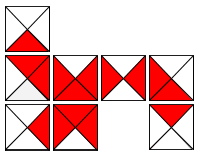
\includegraphics[scale=0.5]{zones connexes.png}
\captionof{figure}{Exemple de zone connexe}
\label{fig : zone}
\end{figure}

Une zone connexe est donc un ensemble de tuiles liées par une couleurs, entre deux tuiles les triangles de même couleur doivent avoir une arête en commun tandis qu'au sein d'une même tuile cette règle n'a pas d'importance. \\

Nous n'avons pas eu le temps de réaliser cet achievement mais voici les idées que nous avions pour l'implémenter. \\

D'après les règles qui définissent une zone connexe nous n'avons pas besoin d'effectuer de tests de connexité de triangles à l'intérieur d'une tuile, nous devons juste faire des tests entre les tuiles. Les tests seront fait à la fin de la partie au même moment que les tests sur les motifs. \\

Pour effectuer ces tests nous pensons qu'il serait judicieux de rajouter un tableau de 4 booléens dans la structure \emph{board\_cell}, celui-ci représenterait les quatre directions d'une tuile. Ainsi, si le booléen en indice \emph{NORTH} est \emph{TRUE} (1 en langage C) alors cela signifie que le triangle dans la direction \emph{NORTH} de la tuile est déjà engagé dans une zone connexe, cela évite de compter plusieurs fois chaque zone connexe .\\

Les tests seraient effectués comme pour le positionnement d'une tuile c'est à dire qu'il y aurait une fonction \emph{test\_connexity} qui prend en argument un plateau de jeu, une coordonnée et une direction, qui trouve la zone connexe et change la valeur des booléens de la \emph{board\_cell} associée. Pour effectuer ces tests on utiliserait un tableau qui serait rempli d'un couple (coordonnées, direction) ce tableau ainsi que sa taille seraient renvoyés par la fonction. La première tuile d'une zone connexe serait mise dans le tableau avec l'une de ces directions (en effectuant d'abord le test sur le booléen pour savoir si ce triangle n'est pas déjà engagé dans une zone connexe). On testerait d'abord si d'autres directions de cette tuile correspondent à la couleur puis on testerait les tuiles connexes à ces directions, si elles ont la même couleur on mettrait le couple (coordonnées, direction) associées dans le tableau puis on ferait les mêmes tests en continuant de parcourir le tableau (sans oublier de changer les booléens pour éviter de compter plusieurs fois un même triangle). \\

La fonction \emph{test\_connexity} serait mise dans la boucle d'une fonction \emph{connexity\_areas} qui appellerait cette fonction pour chaque direction de chaque tuile du plateau. Après l'appel de la fonction \emph{test\_connexity}, elle regarderait d'après le tableau renvoyé quel est le joueur qui a le plus de tuiles ou bien les joueurs s'il y a une égalité. Puis elle distribuerait le score aux joueurs concernés. 

\subsection{Nouvelles règles}
Afin de rendre une partie encore plus intéressante, nous avons pensé à l'ajout de certaines règles. Par exemple, les joueurs pourraient remplacer une tuile déjà présente sur le plateau de jeu si leur tuile peut se placer à la même position tout en respectant les règles de connexité et contiguïté. Cependant, si un joueur remplace une des tuiles, alors il doit prendre celle qu'il a enlevé du plateau dans son deck. Cela amène des stratégies, pour la création de motifs par exemple. Le programme remplacerait alors une tuile si et seulement si cela crée plus de points pour le joueur concerné. Il faudrait donc compter les points au fur et à mesure de la partie. Cela entraînerait une évolution intéressante du code. \\

\'Egalement, il serait possible de rajouter de l'aléatoire dans la création des tuiles, dans les couleurs. Par exemple, il y aurait des couleurs choisies aléatoirement parmi une liste de couleurs, et des tuiles créées aléatoirement avec ces couleurs choisies. \\

Il existe ainsi de nombreuses améliorations possible, comme celles proposées par les achievements 3, 4 et 5.

\section{Conclusion} 
La réalisation du projet Tillings, nous a permis de manipuler de multiples types (structures, pointeurs de fonctions, pointeurs void, etc...) que nous n'avions pas l'habitude d'utiliser. De plus, nous avons découvert la force de la compilation séparée pour l'organisation du code, et la rapidité de recherche d'erreurs ou de parties de code. \\

Ce projet a ainsi été l'occasion de mettre en pratique les notions apprises lors du cours de programmation impérative mais également celles du cours d'algorithmique, d'environnement de travail et de structures arborescentes. Ce fut également l'occasion d'apprendre à programmer à deux en pair-programming ou en parallèle. Pour cela il a fallut communiquer, expliquer avec des mots et non du code la manière dont nous imaginions l'implémentation du jeu. Il a fallut débattre sur nos idées afin de se mettre d'accord, et décider des conventions de code à respecter dans l'intégralité des fichiers. \\

Ainsi le projet d'algorithmique et de programmation nous a permis de progresser dans les matières sollicitées et de découvrir de nouvelles méthodes de travail.

\newpage 
\section{Annexes}
\subsection{Code de la fonction \emph{test\_position}}

\begin{centering}
\fbox{
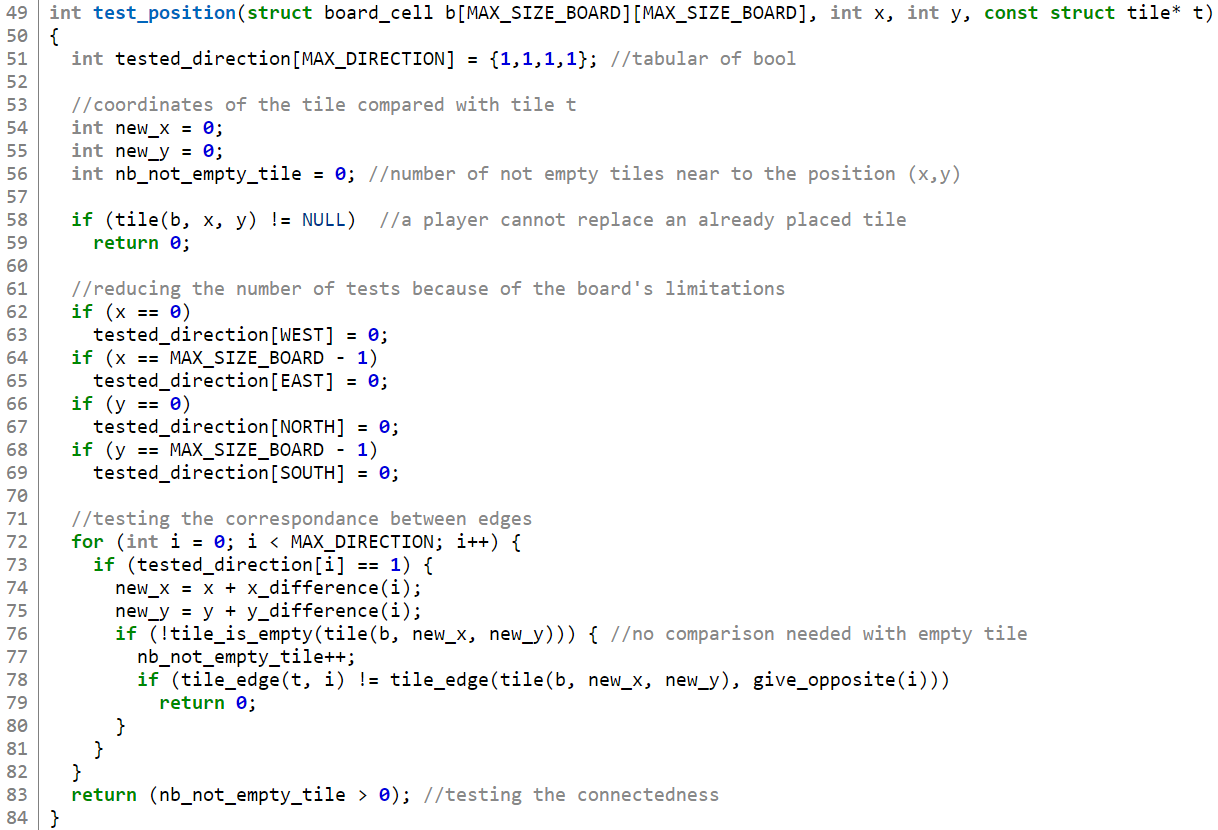
\includegraphics[scale=0.53]{test_position.png}
}
\end{centering}


\subsection{MakeFile} \label{subsec: make}
\begin{centering}
\fbox{
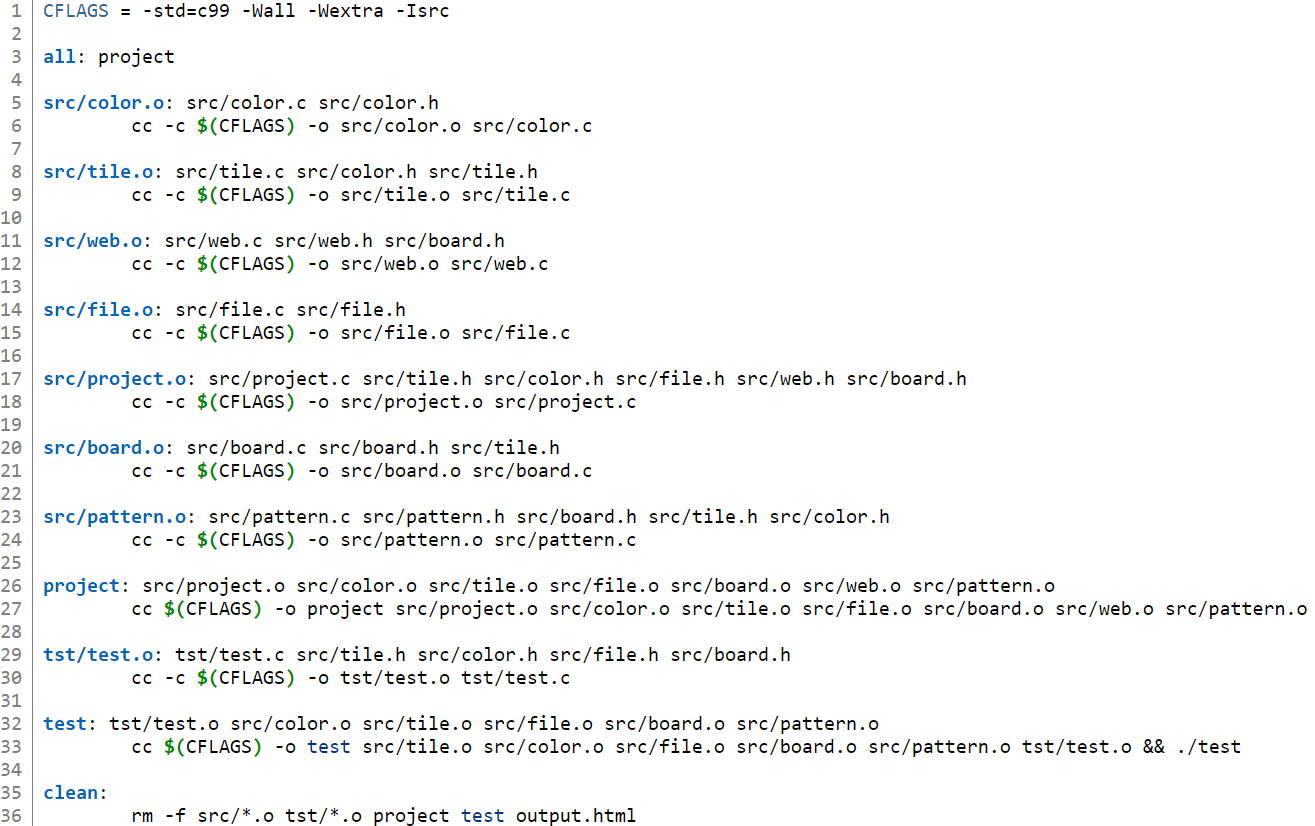
\includegraphics[scale=0.5]{Makefile.png}
}
\end{centering}

\subsection{\'Execution de la commande \emph{make test}} \label{subsec: maketest}

\begin{figure}[H] 
\centering
\fbox{
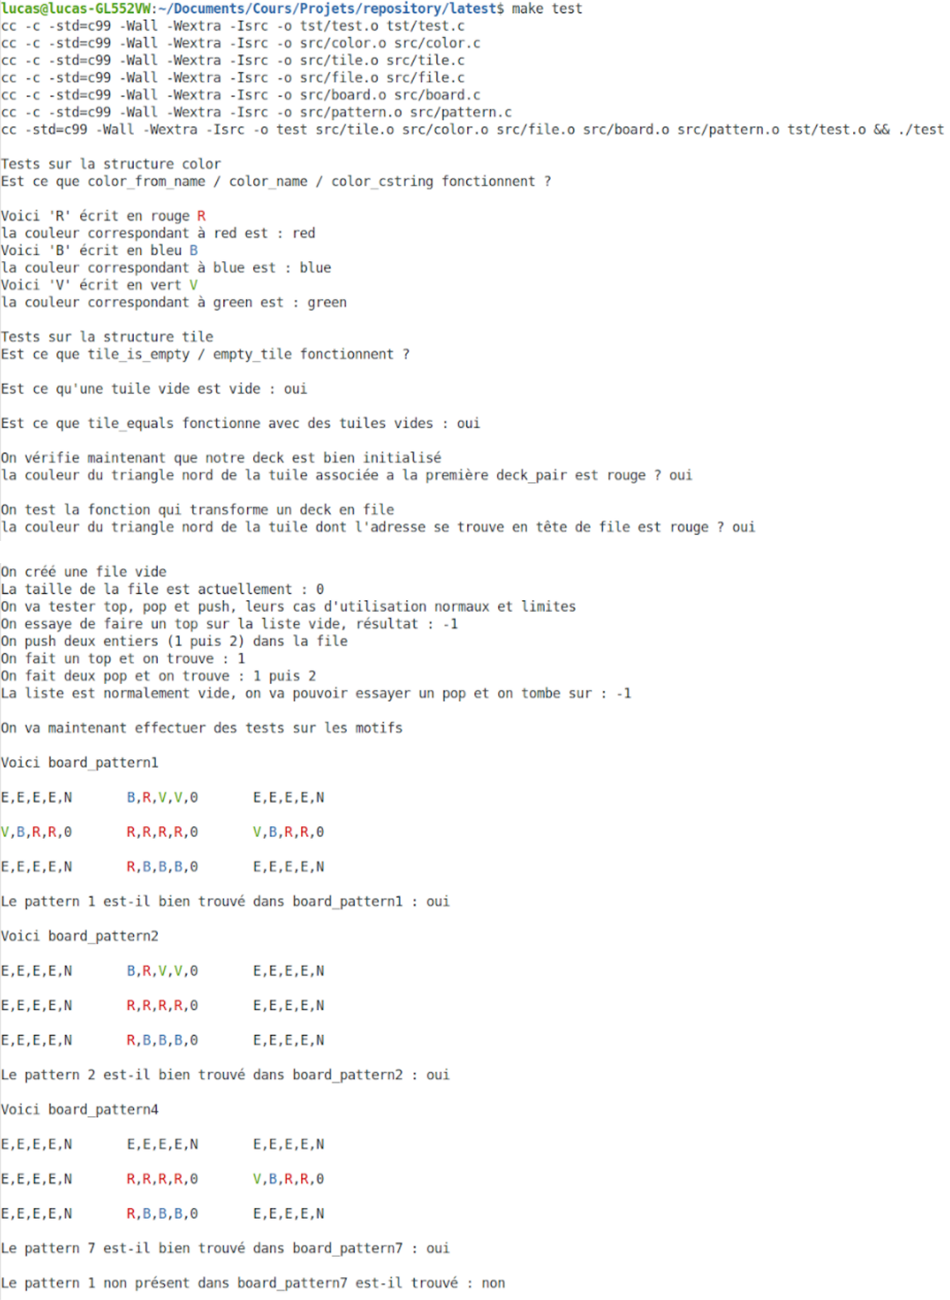
\includegraphics[scale=0.5]{make test.png}
}
\end{figure}

\end{document}


